\section{Formulation of the problem}
\label{Formulation}
%==========================
SPH is a mesh free Lagrange method that starts with the creation of a particle array and is governed by momentum equations, which determine change in density and viscosity. The kernel function $W_{ab}$ is a function of the distance $r_{ab}$ between particle $a$ and $b$.

The interaction between the particle $a$ and the neighboring particles is considered through a smoothening kernel function. In the current paper we used cubic spline kernel .... (see equation \ref{kernel}), where $h$ is the... and $q=r_{ab}/h$ represents the normalized distance between the particle $a$ and $b$. Figure \ref{kernel_figure} show a schematic representation of the kernel function.....


\begin{figure}[h]
\centering
\subfigure[We should redraw this]{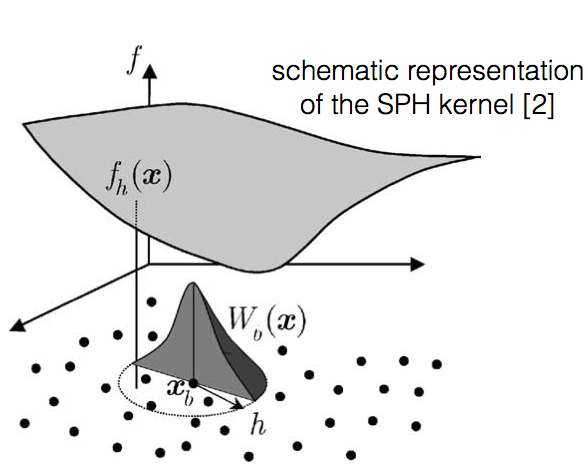
\includegraphics[width=0.5\linewidth]{./_Figures/Kernel.jpg} } 
\subfigure[another generic picture explaining the formulation ]{
\includegraphics[width=0.2\linewidth]{./_Figures/slug.jpg} } 
\caption{array of soft compressible viscoelastic polymer fibers compressed by an elastic wall – the colors represent non-dimensional particle density, where ”1” is the density of the undeformed fibers}
\label{kernel_figure}
\end{figure}


\begin{align}
\label{kernel}
W(r,h)=
\begin{cases}
\frac{10}{7 \pi h^2} \left( 1 - \frac{3}{2}q^2 + \frac{3}{4}q^3 \right), \qquad q<1,\\
\frac{5}{14 \pi h^2} \left( 2-q \right)^3, \qquad \qquad 1<q<2,\\
0, \qquad \qquad \qquad \qquad \qquad 2<q
\end{cases}
\end{align}

\begin{subequations}
\begin{align}
\frac{\partial\rho_a}{\partial t}&=\sum_{b=1}^N m_b\left( \vec v_b- \vec v_a\right) \bigtriangledown_a W_{ab},
\label{eq1}\\
\frac{\vec v_a}{\partial t}&=-\sum_{b=1}^N m_b\left( \frac{p_a}{\rho_a^2}+\frac{p_b}{\rho_b^2}\right) \bigtriangledown_a W_{ab},
\label{eq2}\\
\frac{\vec x_a}{\partial t}&=\vec v_a,
\label{eq3}
\end{align}
\end{subequations}

where $N$ is the total number of particles at distance $|\vec x_a-\vec x_b|<h$, $\rho_i$ is the density, $m_i$ the mass and $\vec v_i$ the velocity of a particle $i \in \{a,b\}$. $\bigtriangledown W$ is the gradient of a smoothing kernel function, $p$ is the pressure applied on a particle, {\color{red} which is obtained from the energy equation. If the SPH method is used to model a fluid, this is given by Tait equation. If, however, a solid is modeled, the pressure is predicted by teh material constitutive model.}

Therefore, for an elastic solid, equation \ref{eq2} could be rewritten as:

\begin{equation}
\frac{\partial v_a^i}{\partial t}=\sum_{b=1}^N m_b\left( \frac{\sigma_a^{ij}}{\rho_a^2}+\frac{\sigma_b^{ij}}{\rho_b^2}+\Pi_{ab}\delta^{ij}\right) \frac{\partial W_{ab}}{\partial x_a^i} +g^i,
\label{eq2_2}
\end{equation}

where $\sigma^{ij}$ is teh stress tensor, the term $\Pi_{ab}\delta^{ij}$ represents teh shear bulk viscosity and $g^i$ is the $i^{\text{th}}$ component of teh body force per unit mass.


%\begin{align}
%\mu(y)=
%\begin{cases}
%\mu_1e^{\alpha y}, \qquad -h\leq y\leq 0,\\
%\mu_0, \qquad -\infty<y<-h
%\end{cases}
%\end{align}

%\begin{subequations}
%\begin{align}
%\frac{\partial\sigma_{xx}}{\partial x}+\frac{\partial\sigma_{xy}}{\partial y}&=0,\label{equil_1}\\
%\frac{\partial\sigma_{xy}}{\partial x}+\frac{\partial\sigma_{yy}}{\partial y}&=0.\label{equil_2}
%\end{align}
%\end{subequations}

%\begin{align}
%\sigma_{yy}(x,0)&=P(x),\notag\\
%\sigma_{xy}(x,0)&=0,
%\end{align}


